%

\documentclass[UTF8]{ctexbook}

\ctexset{
    part/number = \chinese{part}% 用于解决 part 的标号不显示问题
}
\usepackage{hyperref}% 超链接
\hypersetup{
    colorlinks=false,% 去掉超链接颜色
    pdfborder=0 0 0% 取消超链接的边框
}
\usepackage{graphicx}% 图片管理
\graphicspath{{images/}}% 设置图片搜索路径
\usepackage{float,varwidth}% 浮动体
\usepackage{booktabs}% 三线表
\usepackage{tabularx}% 让表格自适应宽度与自动换行
\newcolumntype{Y}{>{\centering\arraybackslash}X}% 定义自适应列的居中格式 Y, 用 X 为左对齐(自适应列)
\usepackage{fancyhdr}% 页眉设置
\usepackage{xcolor}% 颜色宏包
\usepackage{listings}% 代码高亮
\definecolor{codegreen}{rgb}{0,0.6,0}
\definecolor{codegray}{rgb}{0.5,0.5,0.5}
\definecolor{codepurple}{rgb}{0.58,0,0.82}
\definecolor{backcolour}{rgb}{0.95,0.95,0.92}
\lstset{
    commentstyle=\color{codegreen},
    keywordstyle=\color{magenta},
    stringstyle=\color{codepurple},
    basicstyle=\footnotesize,% 代码字体大小
    breakatwhitespace=false,% 是否只在空白字符处断行
    breaklines=true,% 自动断行
    captionpos=b,% 标题位置为 bottom
    keepspaces=true,
    numbers=left,% 行号的位置
    numbersep=5pt,% 行号与代码的距离
    numberstyle=\tiny\color{codegray},% 行号样式
    stepnumber=2,% 隔行显示行号
    showspaces=false,
    showstringspaces=false,
    showtabs=false,
    tabsize=2
}

\begin{document}
  \chapter{开发流程}
    \label{chap:开发流程}

  \section{总体开发流程}
    \label{sec:总体开发流程}
      本次的项目采用 AngularJS 框架开发,AngularJS 项目一般由入口页、模板、控制器、路由控制以及静态资源几大模块构成。大体而流程是: 路由配置 -> 模板设计 -> 数据构造 -> 控制器配置,这些模块的编写没有严格的顺序,模块间是由关联的,因此,改动了一个模块,其他关联的而模块都要跟着改动,

    \subsection{项目结构}
      \label{subsec:项目结构}
                         aystore
                          |
                          |---css/ // CSS 静态资源
                          |    |---artdetail.css
                          |    |---artlist.css
                          |    |---botbar.css
                          |    ...
                          |
                          |---img/ // 主要是一些图标
                          |    |---alipay.png
                          |    |---home.jpg
                          |    ...
                          |
                          |---js/ // js 静态资源
                          |    |---artetail.js
                          |    |---city.js
                          |    |---index.js
                          |    ...
                          |
                          |---less // less 文件,用于编译成 CSS
                          |---node_modules // 项目用到的模块, 如 AngularJS
                          |---res // 存放一些资料,如设计图,方案规划等,不属于项目
                          |---tpl // 模板文件
                          |    |---artdetail.html
                          |    |---ayculture.html
                          |    |---pay.html
                          |    ...
                          |---app.js   // 控制器入口,路由控制,控制器代码
                          |---index.js // 视图入口,html 基本结构,静态资源的一次性引入

      CSS 文件用来控制页面的样式
      入口页负责引入页面的基本框架、静态资源以及视图入口。页面的基本框架即 html, head 和 body 标签。head 标签中配置页面的编码 charset, 移动端兼容以及 CSS 样式文件。

    下面来我们来分析一下有关路由配置的代码。
      \subsubsection{父路由配置举例}
        \label{subsubsec:父路由配置举例}

        \begin{lstlisting}
          $stateProvider
            .state('main', {
              url: '/main',
              templateUrl: "tpl/main.html",
              views: {
                '': {
                  templateUrl: "tpl/main.html"
                },
                'content@main': {
                   templateUrl: "tpl/home.html"
                },
                'botmenu@main': {
                   templateUrl: "tpl/botmenu.html"
                },
              }
            })
        \end{lstlisting}
        上面的代码是主路由(或者叫父路由)的配置,state() 方法的第一个参数为状态名,或者叫路由名; 第二个参数是一个对象,url 字段表示 "main" 这个路由的路径,templateUrl 表示显示的页面文件,此页面文件的作用是划分视图,这里划分为两个视图,一个对应主要内容,另一个对应底部菜单

      \subsubsection{子路由配置举例}
        \label{subsubsec:子路由配置举例}

  \section{home 页的设计}
    \label{sec:home_页的设计}

    \subsection{功能分析}
      \label{subsec:功能分析}
      首页的设计图如下图所示:
      \begin{figure}[H]
        \centering
        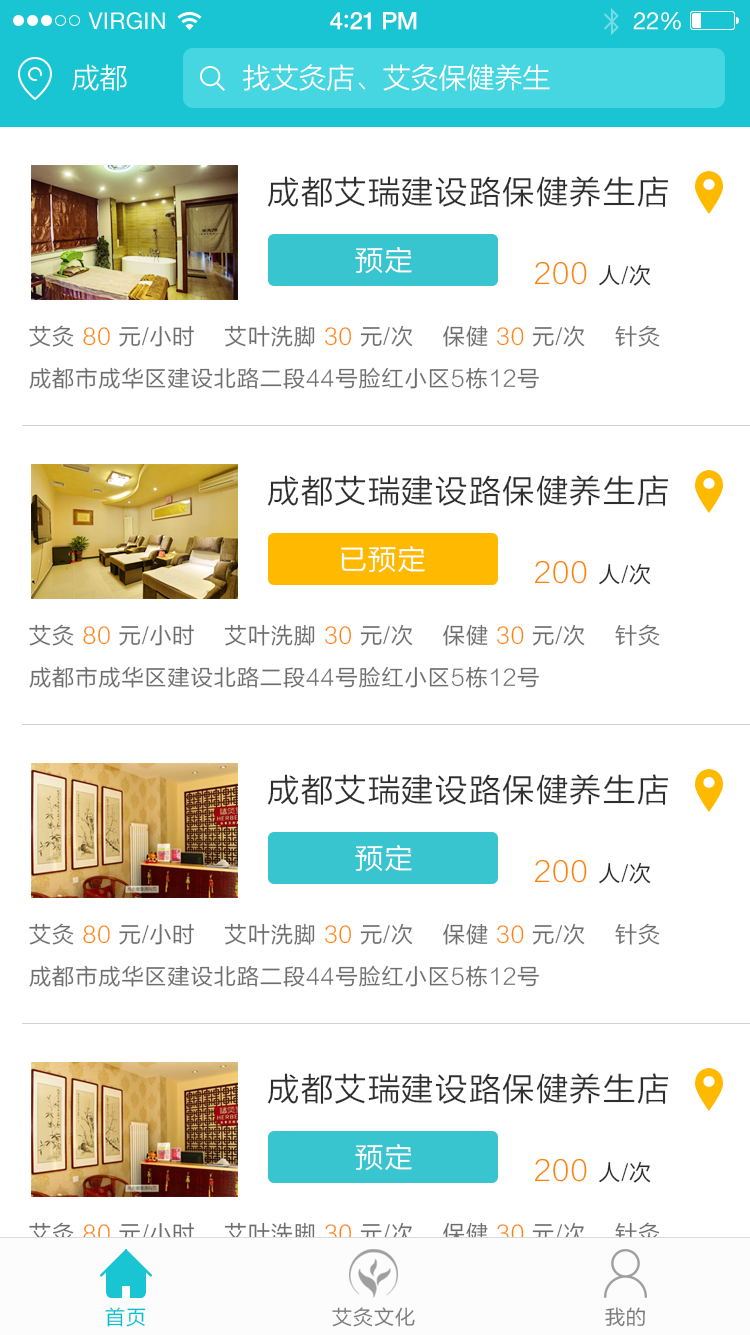
\includegraphics[width=8cm]{img/201705181050.jpg}
        \caption{首页设计图}
        \label{fig:home}
      \end{figure}
      首页主要实现如下功能:
      \begin{itemize}
        \item 地理定位
        \item 商城列表展现
        \item 商城搜索
      \end{itemize}

      \subsubsection{地理定位}
        \label{subsubsec:地理定位功能}
        首次进入商城,(todo)微信接口?还是自己写?应用会自动调用地理定位接口获取客户客户当前的位置,精确到县级,如:成华区,如果定位失败,则返回错误信息,位置自动设置为上一次的位置,并且提醒客户手动定位,点击左上方的按钮
        figtodo: 圈住左上方地理位置选择的图
        就会进入城市选择页,如下图所示:
        figtodo: 城市选择页
        然后就可以选择相应的城市或县区,为了更好地用户体验,如图,还设置了热门城市、最近选择的栏目。

      \subsubsection{列表展现}
        \label{subsubsec:列表展现}
        自动定位(或手动定位)好当前位置后,服务器会返回当前城市的保健店的列表,如图 todo 首页的设计图,简要地展示每个保健店的基本信息,如:店名、缩略图、艾灸床保健价格、其他服务与价格、详细地址以及右上角黄色的地理定位按钮,点击后会应用会打开地图接口,提供更好地体验,如下图:
        figtodo: 店的地图接口
        还有,如果一个店曾经预定过,则会以黄色的按钮提示已预订,点击预定按钮后就会进入店的详情页,展示店的详细信息以及进行预定操作。

      \subsection{商城搜索 todo: 待实现}
        \label{subsec:商城搜索_todo_待实现}
        如图figtodo: 首页设计图,还提供了搜索框,可以根据关键词搜索你想要的店,可以看到搜索框旁边没有搜索按钮,因为搜索是实时显示的,称为增量搜索,而且还采用了自动补全技术,根据最近的搜索关键词和列表加载时自动生成的关键词数据库进行模糊匹配,效果如下:设计非常人性化。
        figtodo: 搜索功能展示

    \subsection{地理定位功能 todo}
      \label{subsec:地理定位功能_todo}

    \subsection{搜索功能 todo}
      \label{subsec:搜索功能_todo}

    \subsection{列表展现}
      \label{subsec:列表展现}
      \subsubsection{数据设计}
        \label{subsubsec:数据设计}
        根据设计图 \ref{fig:home},列表中的每一项展示了如下的信息:
        \begin{itemize}
          \item 缩略图
          \item 店名
          \item 预定状态
          \item 艾灸保健价格
          \item 其他各项服务与价格
          \item 详细地址
        \end{itemize}
        于是我们可以构建如下的 JSON 数据,模拟从数据库提取的数据:
        \begin{lstlisting}
          [
              {
                "strId": "123",// 店的 ID
                "strCity": "成都",// 城市
                "strDistrict": "成华区",// 市区
                "strThumbnail": "http://i2.muimg.com/589268/8aefeb670174ad96t.jpg",// 缩略图
                "strName": "成都艾瑞建设路保健养生店",// 店名
                "ordStatus": 0,// 预定状态,0:已预订,1:未预定
                "strLink": "strlink/store1.html",// todo
                "avgPrice": 200,// 艾灸服务价格
                "srvInfo": "专业技术服务提供服务,智能艾灸床 5 张,艾灸、刮痧、洗脚、按摩、保健、亚健康、养生。",// 描述
                "full": 0,// 是否满员
                // 其他服务的信息
                "strServices": [
                  {
                    "srvName": "艾灸",// 服务名
                    "srvPrice": 80,// 服务价格
                    "srvUnit": "元/小时"// 价格单位
                  },
                  {
                    "srvName": "艾叶洗脚",
                    "srvPrice": 30,
                    "srvUnit": "元/次"
                  },
                  {
                    "srvName": "针灸",
                    "srvPrice": "",
                    "srvUnit": ""
                  }
                ],
                "strMap": "",// todo
                "strAddress": "建设北路二段44号脸红小区5栋12号"// 详细地址
              },
              {
                  "strId": "123",
                  "strCity": "成都",
                  "strDistrict": "成华区",
                  ...
              },
              ...
          ]
        \end{lstlisting}
        缩略图字段是调用的外部的链接,我把图片放到了专门的图片服务器上存储,这样可以节约服务器的空间,这样服务器上不需要再单独开辟一个文件夹盛放图片,也省去了给图片命名的麻烦,也能防止误删、图片文件夹改名的操作导致的图片链接失效。我采用的图片服务器是 “贴图库”,网址为:\url{http://www.tietuku.com/}, 网站虽然样式粗糙,但功能上考虑地很周到,例如可以给图片分组,方便管理,而且可以一键生成图片外链(包括缩略图),点击相应的按钮即可,如图:
        \begin{figure}[H]
          \centering
          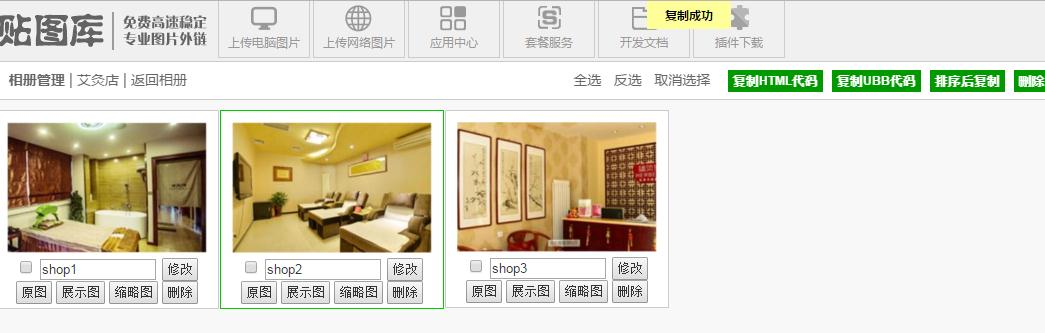
\includegraphics[width=10cm]{./img/tietuku.jpg}
          \caption{贴图库}
          \label{fig:tietuku}
        \end{figure}

      \subsubsection{dom 结构与 CSS 样式设计}
        \label{subsubsec:dom_结构与_css_样式设计}



      \subsubsection{控制器,路由}
        \label{subsubsec:控制器_路由}





















\end{document}
